\Problem
{نتایج}
{
با اجرای برنامه و به دست آمدن مقدار صحیح کلید یعنی مقادیر
\lr{a} و \lr{k}
و اسپیس گذاری اتوماتیک صحیح به متن اصلی می‌رسیم.

\begin{figure}[H]
    \centering
    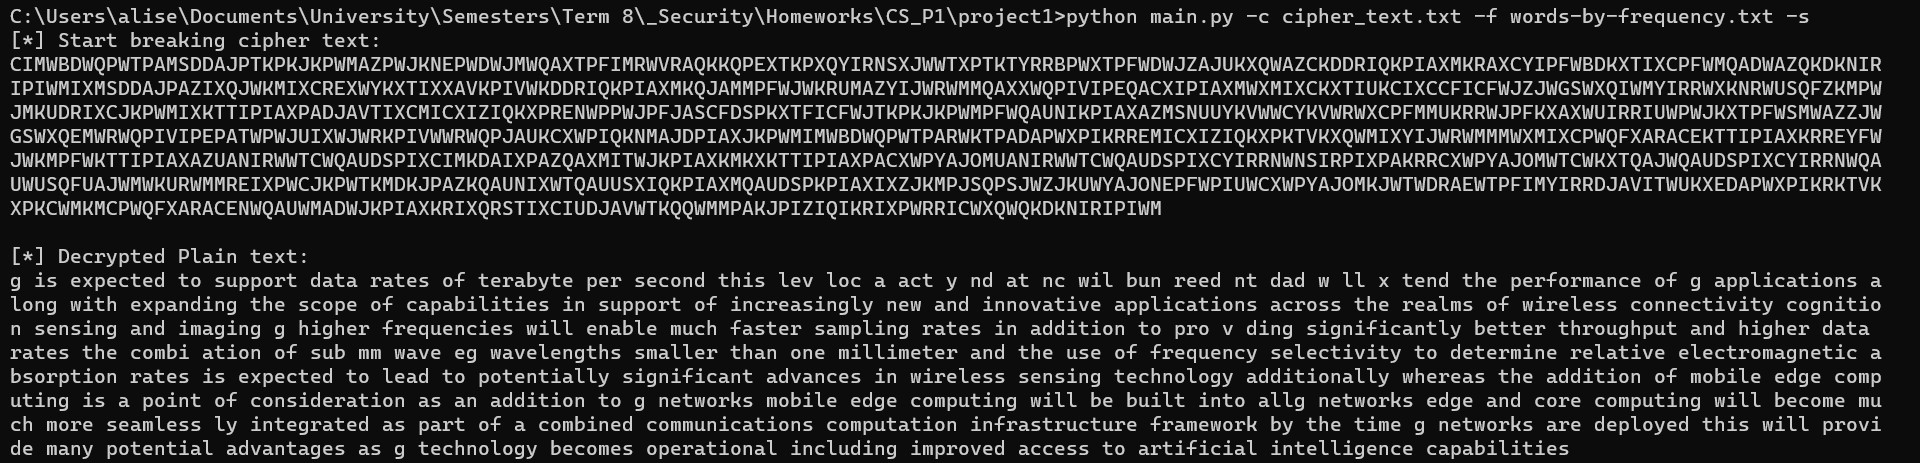
\includegraphics[width=15cm]{Images/Output.jpg}
    \label{fig:label}
    \caption{خروجی برنامه}
\end{figure}

این متن به صورت زیر است:

\lr{
g is expected to support data rates of terabyte per second this level of capacity and latency will be unprecedented and will extend the performance of g applications along with expanding the scope of capabilities in support of increasingly
new and innovative applications across the realms of wireless connectivity cognition sensing and imaging g higher frequencies will enable much faster sampling rates in addition to providing significantly better throughput and higher data rates the combination of sub mm wave eg wavelengths smaller than one millimeter and the use of frequency selectivity to determine relative electromagnetic absorption rates is expected to lead to potentially significant advances in wireless sensing technology additionally whereas the addition of mobile edge computing is a point of consideration as an addition to g networks mobile edge computing will be built into all g networks edge and core computing will become much more seamlessly integrated as part of a combined communications computation infrastructure framework by the time g networks are deployed this will provide many potential advantages as g technology becomes operational including improved access to artificial intelligence capabilities
}

نکته: برخی از خطاهایی که در تصویر آورده شده است بدلیل فاصله گذاری اشتباه الگوریتم بوده است. که به سادگی می‌توان آن‌ها را به صورت دستی اصلاح کرد. با توجه به توضیحات استاد نیازی به اسپیس گذاری صحیح نبود اما این بحش نیز توسط ما پیاده‌سازی شد.
همچنین استفاده از روش
\lr{wordninja}
برای اسپیس‌گذاری نتیجه بهتری خواهد داشت.
}
